\documentclass[UTF8,zihao=-4,a4paper]{ctexart}
\usepackage[a4paper,margin=2.28cm,headheight=14pt,footskip=1.1cm]{geometry}
\usepackage{amsmath,amssymb,mathtools,booktabs,array,tabularx,longtable}
\usepackage{graphicx,caption,subcaption,float,placeins}
\usepackage{hyperref,xcolor,fancyhdr,enumitem,lastpage}
\usepackage{microtype}
\setCJKmainfont{Noto Serif CJK SC}
\setCJKsansfont{Noto Sans CJK SC}
\setmainfont{Liberation Serif}
\setsansfont{Liberation Sans}
\setmonofont{DejaVu Sans Mono}[Scale=0.82]
\definecolor{ink}{HTML}{1D3045}
\definecolor{accent}{HTML}{19537A}
\definecolor{soft}{HTML}{6C7986}
\definecolor{rulec}{HTML}{D0DAE3}
\hypersetup{colorlinks=true,linkcolor=accent,urlcolor=accent,citecolor=accent,pdftitle={DANDI 000138 四维 Hard HiWA 实验与问题诊断},pdfauthor={项目实验记录}}
\ctexset{section={format=\Large\bfseries\color{ink},beforeskip=18pt,afterskip=10pt},subsection={format=\large\bfseries\color{accent},beforeskip=12pt,afterskip=6pt}}
\renewcommand{\arraystretch}{1.22}
\setlength{\parindent}{2em}
\setlength{\parskip}{3pt}
\setlist[itemize]{leftmargin=2.5em,itemsep=2pt,topsep=3pt}
\captionsetup{font=small,labelfont={bf,color=ink},labelsep=quad}
\graphicspath{{results/clustering/}{results/hard_hiwa/}{results/diagnostics/}}
\pagestyle{fancy}
\fancyhf{}
\fancyhead[L]{\footnotesize\color{soft}DANDI:000138 · 四维 Hard HiWA}
\fancyhead[R]{\footnotesize\color{soft}实验技术报告 / 2026-11-17}
\fancyfoot[C]{\footnotesize\color{soft}\thepage\ / \pageref{LastPage}}
\renewcommand{\headrulewidth}{0.35pt}
\newcommand{\repo}{\href{https://github.com/noelabernathy400-bot/ot-hiwa/tree/main/projects/dandi-000138-hiwa-4d}{GitHub 项目目录}}
\newcommand{\R}{\mathbb{R}}
\newcommand{\fro}{\mathrm{F}}
\newcommand{\dataseturl}{\url{https://dandiarchive.org/dandiset/000138/0.220113.0407}}
\begin{document}
\begin{titlepage}
\thispagestyle{empty}
\vspace*{2.2cm}
{\sffamily\color{accent}\Large 应用数学研究 · 可复现实验记录\par}
\vspace{0.65cm}
{\Huge\bfseries\color{ink}DANDI 000138 四维数据\par}
\vspace{0.22cm}
{\Huge\bfseries\color{ink}Hard HiWA 对齐实验\par}
\vspace{0.22cm}
{\LARGE\bfseries\color{accent}数据、方法、结果与失败原因诊断\par}
\vspace{1.2cm}
{\noindent\color{soft}\rule{\linewidth}{1pt}\par}
\vspace{0.65cm}
\begin{tabular}{@{}ll@{}}
数据源 & DANDI:000138 / MC\_Maze\_Large \\
数据版本 & \texttt{0.220113.0407} \\
算法版本 & 用户压缩包内原版 PyHiWA（代码不改） \\
维度与分组 & 神经 4D / 手部运动 4D；独立 K-means，$K=4$ \\
数据划分 & 400 训练试次 / 100 留出测试试次 \\
实验日期 & 2026 年 11 月 17 日 \\
状态 & 硬聚类和 Hard HiWA 完成；几何假设存在明显不匹配 \\
\end{tabular}
\vfill
\noindent\fcolorbox{rulec}{white}{\parbox{0.94\linewidth}{\small\bfseries 核心发现\quad\normalfont
五次 Hard HiWA 均满足数值审计，但测试集 $R^2$ 全为负值。使用同一四维输入的有监督 Ridge 线性映射却达到 $R^2\approx0.287$；在固定运动评价窗口中，训练验证选出的 $+140\,\mathrm{ms}$ 时间偏移进一步提高至 $R^2\approx0.390$。这更支持\textbf{正交几何假设、时间配准和簇质量设定有问题}，而非 ``神经数据完全没有运动信息''。}}
\vspace{0.7cm}
{\small\color{soft}项目地址：\repo\par}
\end{titlepage}

\tableofcontents
\newpage
\section{研究问题与报告范围}
本项目的研究对象是\textbf{无监督神经活动--手部运动分布对齐}：神经活动从高维放电表征映射至四维潜在空间，手部运动域保留原本的四个连续观测量，然后独立硬分组并用原版 Hierarchical Wasserstein Alignment（HiWA）学习跨域正交映射。

我们希望回答三个层次分明的问题：
\begin{enumerate}[leftmargin=2.5em,itemsep=4pt]
\item 两个四维域各自是否存在可识别的分组结构？
\item 原版 Hard HiWA 在数值上收敛以后，是否能够找到有意义的跨域簇匹配和正交矩阵？
\item 这种无监督分布对齐是否能解释\emph{同一试次、同一时刻}的实际运动行为？如果不能，主要障碍是算法优化、特征表示还是模型假设？
\end{enumerate}
本文在保留既有聚类及 HiWA 结果的基础上进行诊断。\textbf{所有新增的监督线性回归、时间偏移分析和簇共现分析均为诊断实验，绝不是 HiWA 的训练步骤，也不应与 HiWA 的效果混为一谈。}

\section{数据来源与记录内容}
\subsection{官方数据源}
使用 DANDI Archive 的 Dandiset \textbf{000138}，发布版本 \texttt{0.220113.0407}，名称 \emph{MC\_Maze\_Large: macaque primary motor and dorsal premotor cortex spiking activity during delayed reaching}，DOI：\href{https://doi.org/10.48324/dandi.000138/0.220113.0407}{10.48324/dandi.000138/0.220113.0407}。官方发布页面见\,[1]；数据集属于 Neural Latents Benchmark (NLB) 的运动皮层延迟伸手任务家族\,[2,3]。

实验为恒河猴执行有视觉障碍物的延迟到达任务。在 M1（初级运动皮层）和 PMd（背侧前运动皮层）记录放电，同时记录手部及光标运动变量。\textbf{这里是侵入式运动皮层神经放电数据，不是 Hyser 的肌电数据，也不是单独控制五根手指的施力数据。}

本轮仅使用官方行为与神经活动共同存在的训练 NWB 文件：
\begin{center}
\ttfamily\small sub-Jenkins\_ses-large\_desc-train\_behavior+ecephys.nwb
\end{center}
另一测试文件含有不同程度的缺失行为信息；为了能够进行真实同步行为评价，本项目在上述训练 NWB 的 \textbf{500 个可用试次内部}，按试次重新划分训练 400 个与留出测试 100 个。请不要与 NLB 官方隐藏测试集的划分混淆。

\begin{table}[H]\centering\small
\caption{数据集与本次实验的固定输入}\label{tab:data}
\begin{tabular}{@{}p{5.5cm}p{8.5cm}@{}}\toprule
项目 & 内容\\\midrule
数据及版本 & DANDI:000138 / 0.220113.0407\\
实验神经元数 & 162 个单元（NWB \texttt{units} 表）\\
行为向量 & $y(t)=(p_x(t),p_y(t),v_x(t),v_y(t))\in\R^4$\\
运动参照时刻 & 试次的 \texttt{move\_onset\_time}\\
每试次取样区间 & $[-100,600]\,\mathrm{ms}$，每个时窗 20\,ms\\
每试次窗口数 & 35\\
训练/测试 & 400 / 100 个试次，合计 14,000 / 3,500 个窗口\\
分组及随机种子 & $K=4$，分组 seed = 42\\\bottomrule
\end{tabular}
\end{table}

\section{从 NWB 到四维源域和目标域}
\subsection{神经源域：162 维放电到四维 PCA}
记第 $u$ 个神经元的 spike times 为 $\{t_{u,k}\}$。在宽度 $\Delta t=0.02\,\mathrm{s}$ 的非重叠时窗 $I_j$ 内，先计算放电率
\begin{equation}
 z_{j,u}=\frac{\#\{t_{u,k}\in I_j\}}{\Delta t},\qquad u=1,\ldots,162.
\end{equation}
随后对非负放电率开平方，并在\textbf{每个试次的时间轴}采用 40\,ms 标准差的 Gaussian 平滑；特征标准化的均值和方差仅由训练试次估计。若标准化后的高维训练矩阵为 $Z_{\mathrm{tr}}$，取其前四个 PCA 主方向 $V_4\in\R^{162\times4}$，得到
\begin{equation}
 x_j=V_4^\top\operatorname{Standardize}(z_j)\in\R^4.
\end{equation}
PCA 仅在训练集拟合，然后原样作用于测试数据。前四个主成分分别解释 4.47\%、3.84\%、2.55\%、2.20\% 的特征方差，累计约 \textbf{13.06\%}。这一比例偏低，值得作为表示能力的疑点；但方差贡献率并不等价于运动解码信息含量。

\subsection{手部运动目标域：保留原本四个坐标}
目标域严格采用 NWB 中记录的手部位置与速度：
\begin{equation}
 y_j=(\mathrm{hand\_pos}_x,\mathrm{hand\_pos}_y,\mathrm{hand\_vel}_x,\mathrm{hand\_vel}_y)\in\R^4.
\end{equation}
行为时间序列按 spike 时窗中心时间做插值。\textbf{目标域没有 PCA、没有进一步降维。} 为避免位置和速度因物理量纲不同而主导 K-means，各个行为坐标仅使用训练集均值与标准差做逐坐标标准化。这一变换不是将其从 4D 降为 3D。

\subsection{HiWA 之前的全局尺度规范化}
硬分组是在上述四维表示中独立完成的。进行 HiWA 拟合之前，再对两域各自减去训练集均值并除以\textbf{单一的 RMS 半径}：
\begin{equation}
 \widetilde x=\frac{x-\mu_X}{s_X},\quad s_X^2=\frac1{N_{\rm tr}}\sum_{i\in\mathrm{tr}}\|x_i-\mu_X\|_2^2,\qquad
 \widetilde y=\frac{y-\mu_Y}{s_Y}.
\end{equation}
该操作统一各域整体尺度，不会对每个维度再做二次白化。但两域采用不同的归一化因子，因此学到的正交矩阵是\textbf{归一化四维空间中的正交映射}，不是在物理单位下直接代表手部运动方程的旋转。

\section{两域最初的四维硬聚类：原始散点图}
分别在 $X,Y\subset\R^4$ 中执行 K-means（$K=4$，\texttt{n\_init=20}，seed = 42），训练集簇数分别为
\begin{equation*}
N_X=(4137,4316,3146,2401),\qquad N_Y=(2818,6316,2012,2854).
\end{equation*}
训练集 Silhouette：神经域 $0.33961$，手部运动域 $0.37032$。这些分数显示一定分组结构，但并非清晰分离的独立子流形。

以下两图\textbf{直接采用第一次真实四维聚类实验输出的原始文件}，每张图覆盖 $\binom42=6$ 组二维坐标投影，\textbf{聚类始终在四维完成，并非在二维完成}。颜色编号在两个域中独立产生，不意味着已经找到簇对应。

\begin{figure}[p]\centering
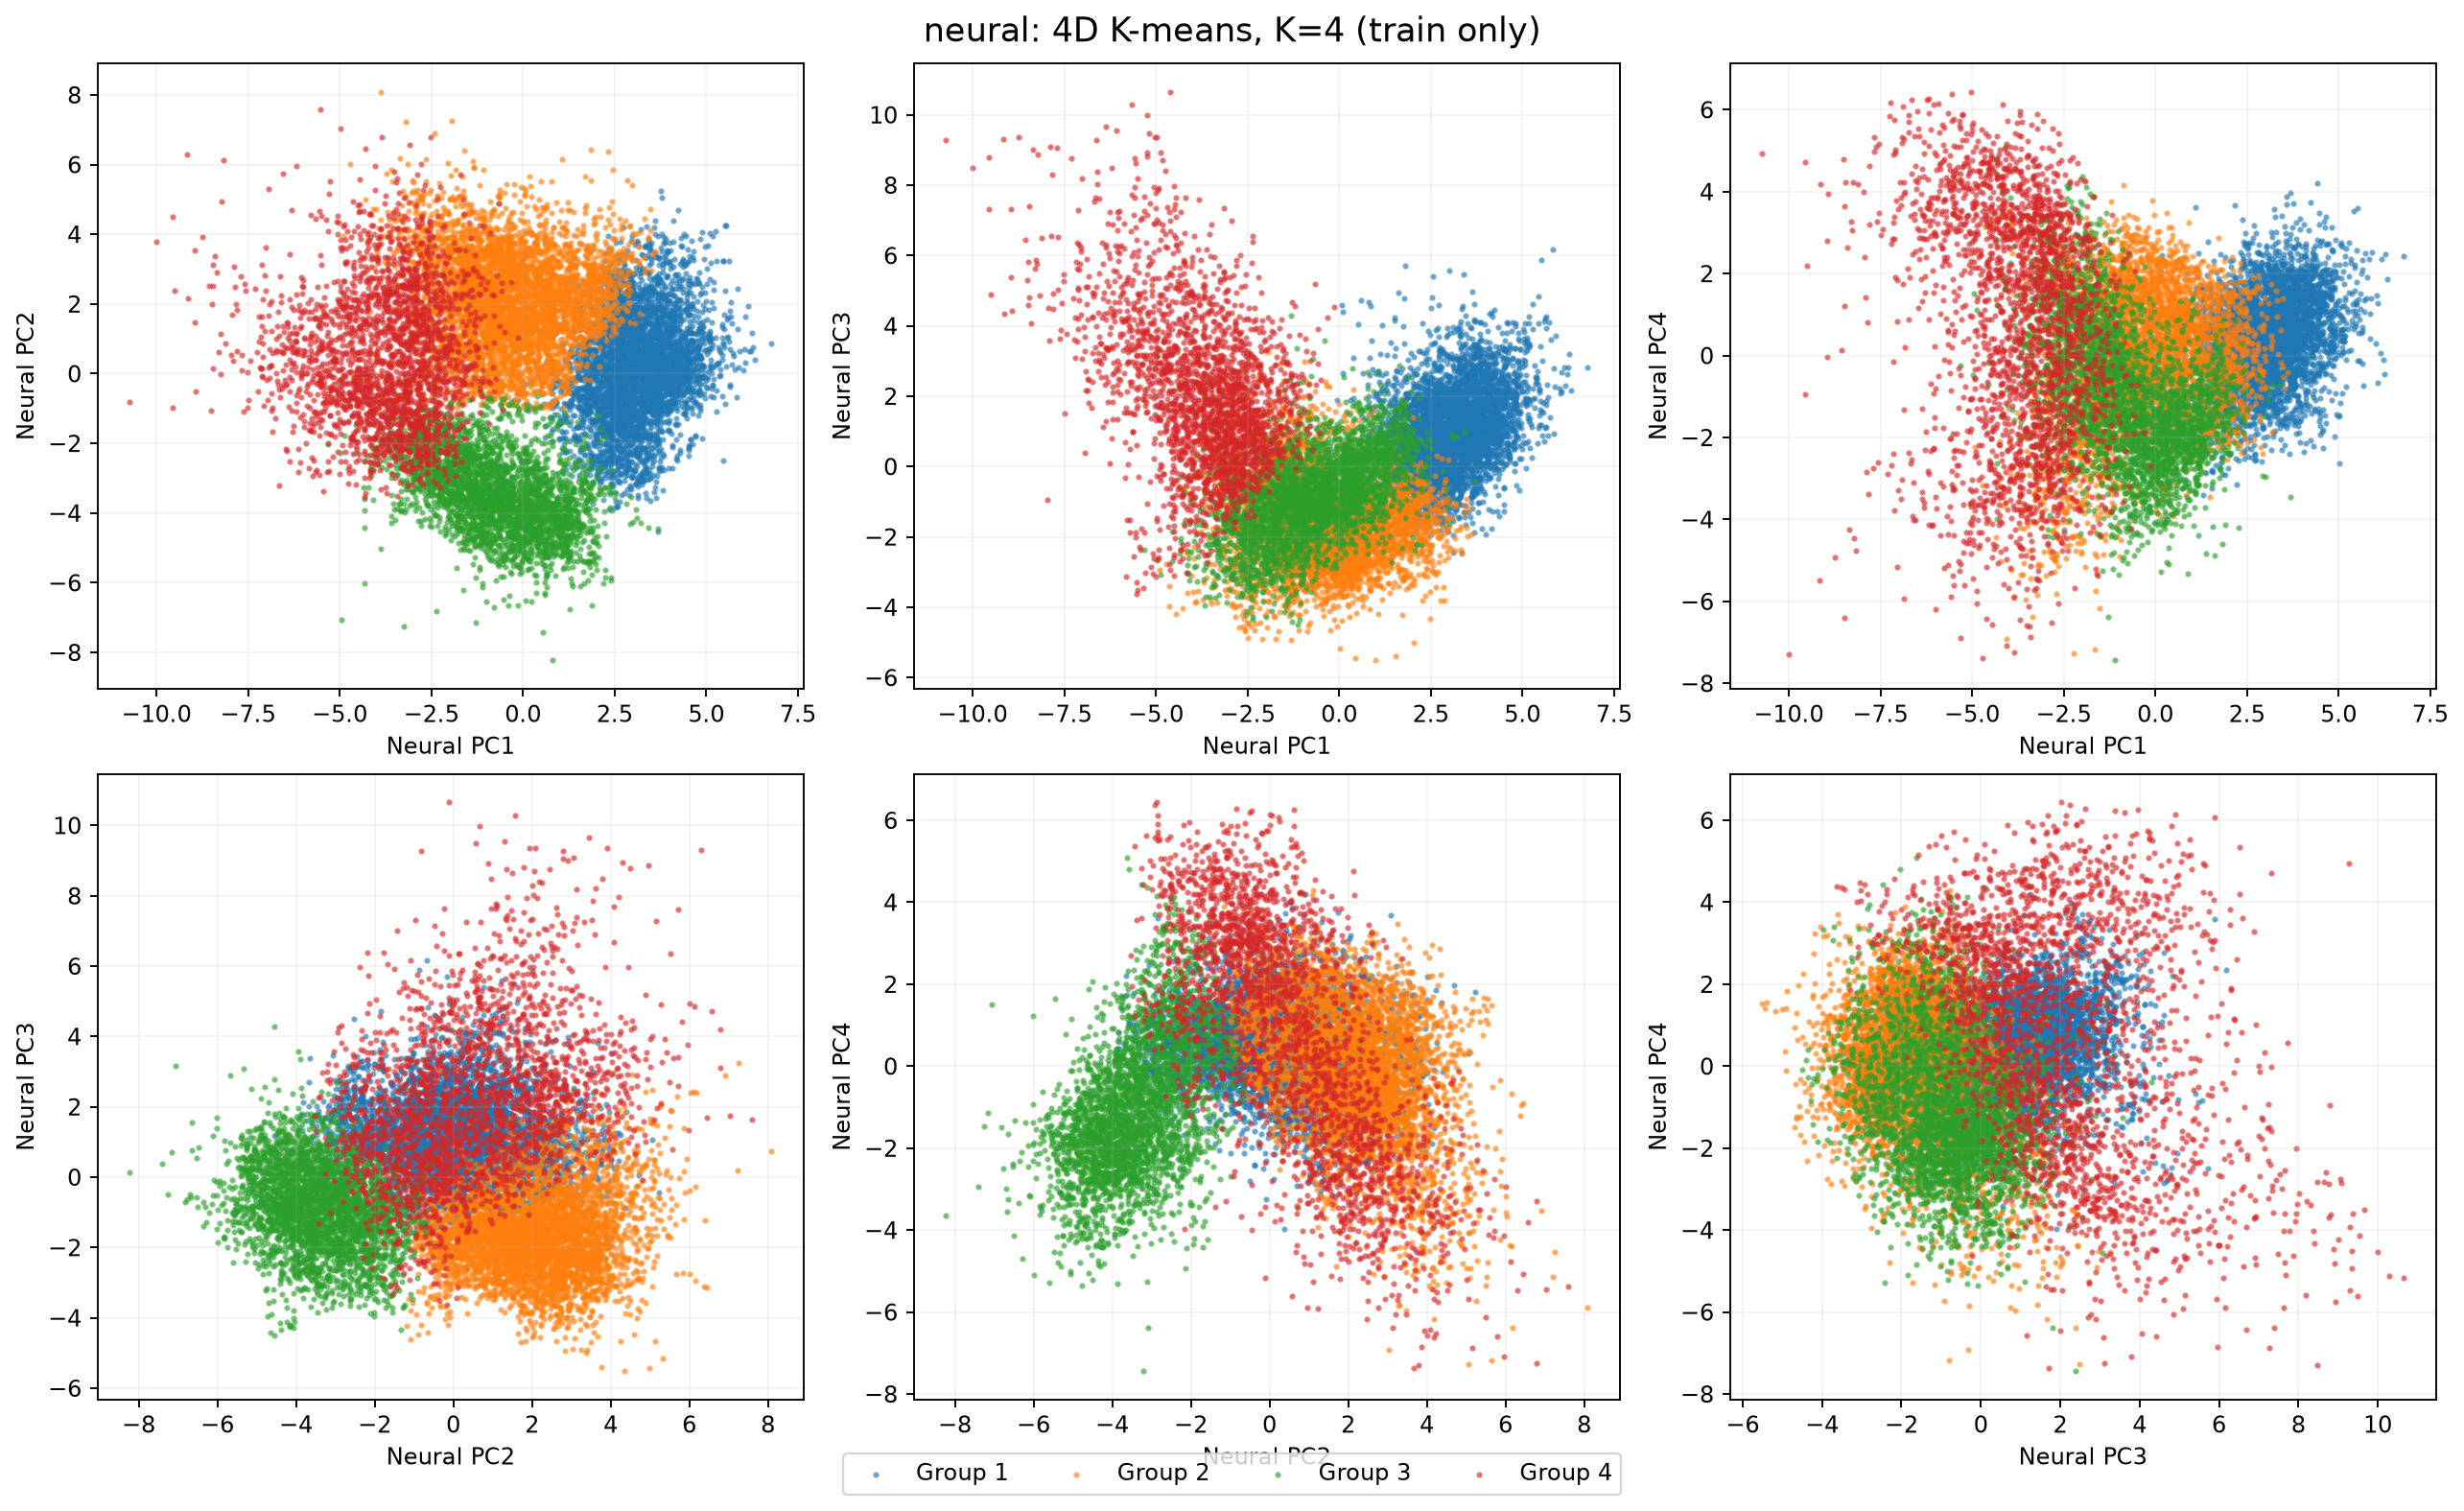
\includegraphics[width=\textwidth]{neural_4d_pairwise_train.png}
\caption{初始神经源域 $X$：四维 PCA 表示上 K-means 的六个二维投影。数据为 14,000 个训练时窗；不同颜色表示神经域内独立得到的四个簇。}\label{fig:source}
\end{figure}
\clearpage
\begin{figure}[p]\centering
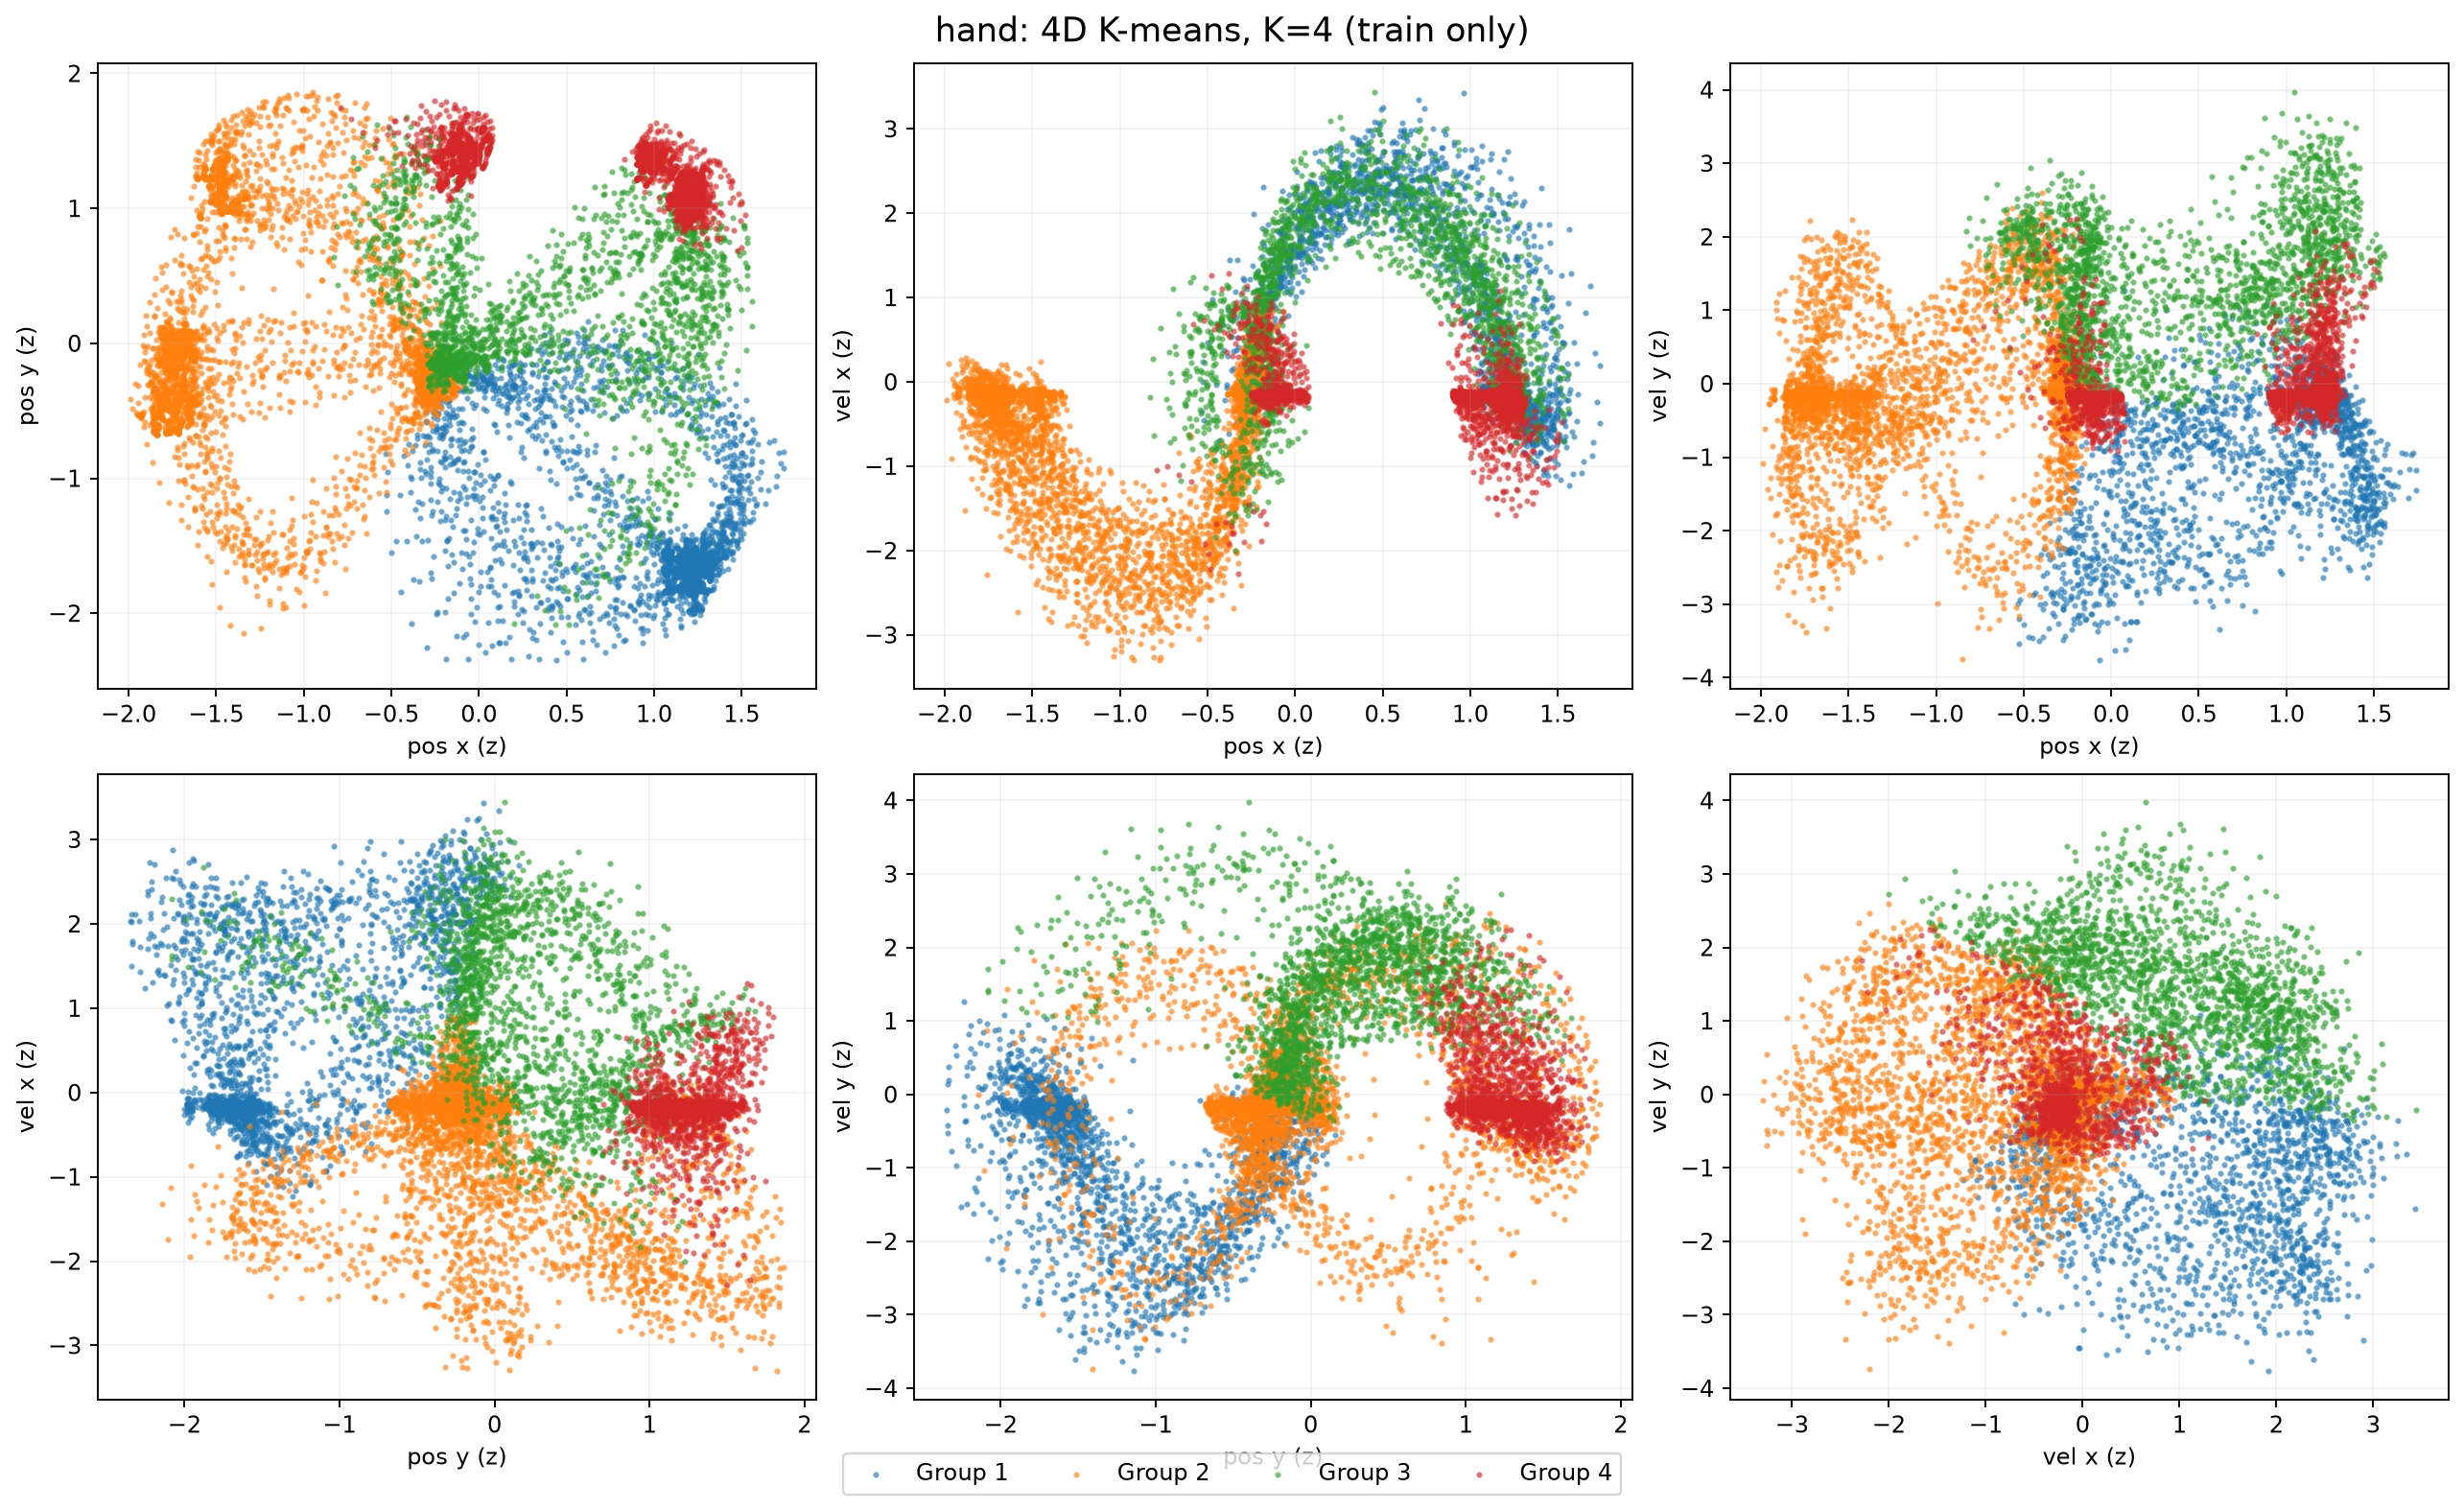
\includegraphics[width=\textwidth]{hand_4d_pairwise_train.png}
\caption{初始手部运动目标域 $Y$：保留 $p_x,p_y,v_x,v_y$ 四维变量后的 K-means 六个二维投影；仅对四个坐标按训练集标准化。目标域没有 PCA。}\label{fig:target}
\end{figure}
\clearpage

\section{原版 Hard HiWA 的实验设计}
\subsection{算法目标与运行设置}
使用用户提供的上传压缩包中的原版 PyHiWA，算法文件为 \path{reference/HiWA/PyHiWA/src/hiwa.py}，本项目保存为 \path{code/hiwa_original.py}。求解器不做算法修改，旧仓库中的其他 HiWA 实现不参与本次复现。

用 $\widehat R\in O(4)$ 表示估计的全局正交矩阵，局部簇对具有 $R_{ij}\in O(4)$；$P\in\R_+^{4\times4}$ 是簇间传输计划。原版算法交替进行局部正交变换、局部 Sinkhorn、簇间 Sinkhorn、全局旋转更新与 ADMM 共识更新。
\begin{equation}
 O(4)=\{R\in\R^{4\times4}:R^\top R=I_4\},\qquad
 P\mathbf1=\tfrac14\mathbf1,\quad P^\top\mathbf1=\tfrac14\mathbf1.
\end{equation}
注意 $O(4)$\textbf{允许行列式 $-1$ 的反射}，而不仅是 $SO(4)$ 旋转。原版用 SVD 的 $UV^\top$ 更新 $R$，并没有强制 $\det R=+1$。

\begin{table}[H]\centering\small
\caption{Hard HiWA 固定超参数（与已归档实验一致）}\label{tab:parameters}
\begin{tabular}{@{}lll@{}}\toprule
参数 & 数值 & 说明\\\midrule
算法随机种子 & 42--46 & 5 次独立初始化\\
每域每簇拟合样本数 & 40 & 每域 160 样本，域间独立抽取\\
最大外迭代 & 140 & ADMM 外循环\\
原版停止阈值 & $10^{-9}$ & 全局矩阵变化\\
额外审计阈值 & $10^{-2}$ & 全局与局部--全局共识\\
$\mu$ & 0.05 & ADMM 系数\\
簇间 Sinkhorn & $\gamma=0.2$, 200 次 & 组级熵正则 OT\\
簇内 Sinkhorn & $\gamma=0.1$, 45 次 & 局部 OT\\
局部交替求解 & 最多 20 次 & 局部停止阈值 0.01\\\bottomrule
\end{tabular}
\end{table}

\subsection{评价口径：只保留 HiWA 中的两个主指标}
原版 PyHiWA 定义了\textbf{相对均方误差 rMSE}：
\begin{equation}\label{eq:rmse}
\mathrm{rMSE}(\widehat R;R_{\rm gt})=
\frac{\|R_{\rm gt}X^\top-\widehat R X^\top\|_F^2}
{\|R_{\rm gt}X^\top\|_F^2}.
\end{equation}
它用于\emph{已知真实旋转} $R_{\rm gt}$ 的设置。\textbf{DANDI 真实神经--行为数据没有 $R_{\rm gt}$。} 因此不能汇报真实 rMSE。我们只以\emph{训练集同步配对最小二乘正交 Procrustes} 的 $R_{\rm ref}$ 代替 $R_{\rm gt}$，得到\textbf{代理 rMSE}，且明确其不是地面真值旋转误差。

第二个指标采用标准的多输出决定系数（总平方和形式）：
\begin{equation}\label{eq:r2}
 R^2=1-\frac{\sum_{i\in\mathrm{test}}\|y_i-\widehat R x_i\|_2^2}
 {\sum_{i\in\mathrm{test}}\|y_i-\bar y_{\rm test}\|_2^2}.
\end{equation}
需特别指出：\textbf{原版 \texttt{\_eval\_R2} 的源码没有使用平方残差}，其返回值不是标准 $R^2$。我们不修改求解器，只在独立评估脚本中修正标准公式。低于零表示比测试集常数均值预测的平方误差更大。原先额外计算的两种 NRMSE 仅作历史记录，\textbf{不再作为本报告的主要质量评价指标}。

\section{正式 Hard HiWA 结果}
\begin{table}[H]\centering\small
\caption{相同留出测试集的两项 HiWA 评价指标。\emph{代理 rMSE 并非真实 rMSE}。}\label{tab:hiwa}
\begin{tabular}{@{}lrr@{}}\toprule
方法 & 代理 rMSE $\downarrow$ & 标准 $R^2$ $\uparrow$\\\midrule
未对齐：$\widehat R=I$ & 1.96470 & $-0.79649$\\
HiWA seed 42 & 2.11824 & $-0.80478$\\
HiWA seed 43 & 1.26308 & $-0.54862$\\
HiWA seed 44 & 2.09887 & $-1.09933$\\
HiWA seed 45 & 1.97163 & $-0.95505$\\
HiWA seed 46 & 2.12925 & $-1.06582$\\
\textbf{HiWA 五次均值 $\pm$ 样本标准差} & \textbf{1.91621 $\pm$ 0.37054} & \textbf{$-0.89472\pm0.22508$}\\
训练集同步配对 Procrustes（诊断） & 0（按参照定义） & $-0.06044$\\\bottomrule
\end{tabular}
\end{table}

原版求解器的五次实验均通过额外的全局、局部共识和组间 OT 边缘审计；但\textbf{数值收敛不意味着找到了可解释的神经--手部运动映射}。五次测试集 $R^2$ 全为负值，且平均略劣于未对齐。最佳正交有监督诊断在测试集上也只有 $R^2=-0.06044$，提示\textbf{问题并不只是 HiWA 的数值迭代次数不足}。

\section{失败原因诊断：用相同四维数据寻找问题}
\subsection{关键诊断 A：并非没有运动信息，而是正交限制过强}
不改变四维输入和测试划分，单独允许训练集同步配对来拟合一个普通的全线性 Ridge 模型
\begin{equation}
 \widehat y=Ax+b,\qquad A\in\R^{4\times4},
\end{equation}
与正交 Procrustes 的 $\widehat y=Rx$ 对比。结果是：
\begin{table}[H]\centering\small
\caption{留出测试集同一时刻的标准 $R^2$：几何映射类型的诊断性比较}\label{tab:diagnosis}
\begin{tabular}{@{}lr@{}}\toprule
映射类型 & 测试 $R^2$\\\midrule
不对齐，直接比较 $x$ 与 $y$ & $-0.7965$\\
无监督原版 Hard HiWA（五次均值） & $-0.8947$\\
有监督、无截距正交 Procrustes & $-0.0604$\\
\textbf{有监督一般线性 Ridge（同样仅四维）} & \textbf{0.2868}\\\bottomrule
\end{tabular}
\end{table}
这里 Ridge 是\emph{需要真实训练配对}的诊断对照，不能称作无监督 HiWA 的改进结果。它表明当前四个神经主成分至少保留了部分可解码信息，且自由线性映射明显优于正交映射：目前最强的证据指向\textbf{单一全局等距/正交几何假设不适合这两个空间}。

训练集四对标准 CCA 相关系数约为 $0.861,0.479,0.241,0.133$，表明跨域线性相关强烈集中在少数方向，并非四个方向都一样强。该结果是相关结构的描述，不是因果关系，也不等于证明存在可逆一一映射。

\begin{figure}[H]\centering
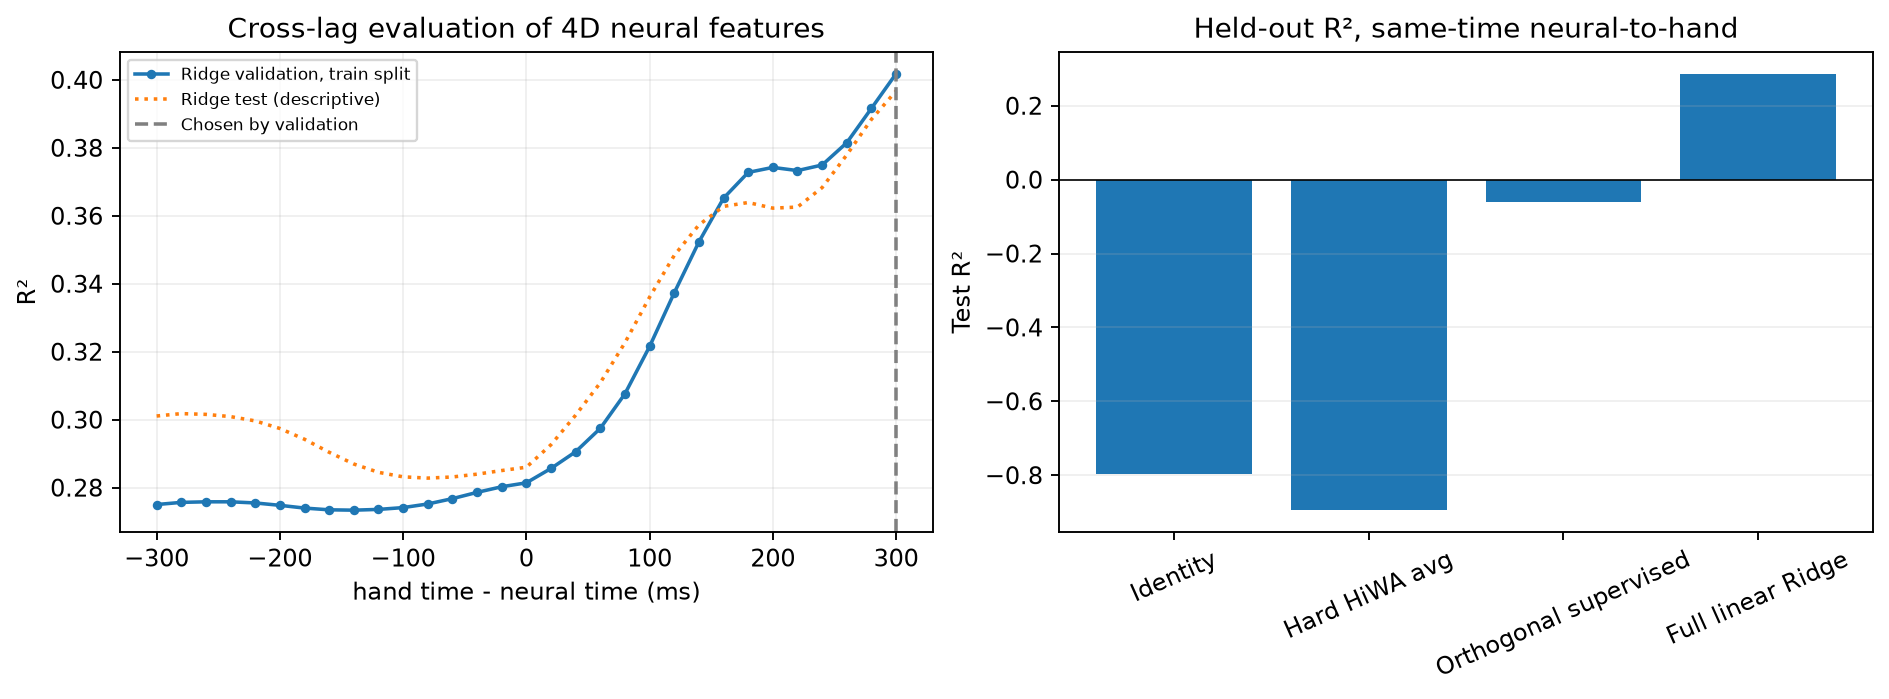
\includegraphics[width=0.96\textwidth]{diagnostic_linear_vs_orthogonal.png}
\caption{左：允许不同预测延迟、且训练验证集择优的探索性扫描，比较的时窗范围随延迟变化，因此不能直接解释为生理时滞；右：同一时刻四维映射类型的 $R^2$ 对照。固定评价窗口的改进分析见图\ref{fig:fixedlag}。}\label{fig:linear}
\end{figure}

\subsection{关键诊断 B：神经与运动可能存在时间错位}
原实验只评价同步时窗 $x(t)\leftrightarrow y(t)$。然而神经放电与手部运动存在任务相关的时序关系。为避免不同延迟改变评价时间段而使分数不可比，我们将\textbf{目标手部运动的时间窗固定为相对运动开始的 $110$--$390\,\mathrm{ms}$}，在所有候选偏移 $\ell\in\{-200,-180,\ldots,200\}\,\mathrm{ms}$ 下比较
\begin{equation}
\widehat y(t)=A_{\ell}x(t-\ell)+b_{\ell}.
\end{equation}
在 400 个训练试次内部再划分模型拟合与验证试次，\emph{只根据训练验证集}选择 $\ell$ 与 Ridge 正则系数，最后评价原先固定的 100 个测试试次。

本次固定窗口诊断得到：验证集最优 $\ell=+140\,\mathrm{ms}$，验证 $R^2=0.3875$，留出测试 $R^2=0.3902$。含义是\emph{较早的神经特征}与\emph{较晚的手部运动}之间存在更强的线性关联。若在留出测试集上打乱试次与行为的对应关系，100 次随机对照的 $R^2$ 平均约 $-0.334$，为关联的非平凡性提供辅助证据。

\begin{figure}[H]\centering
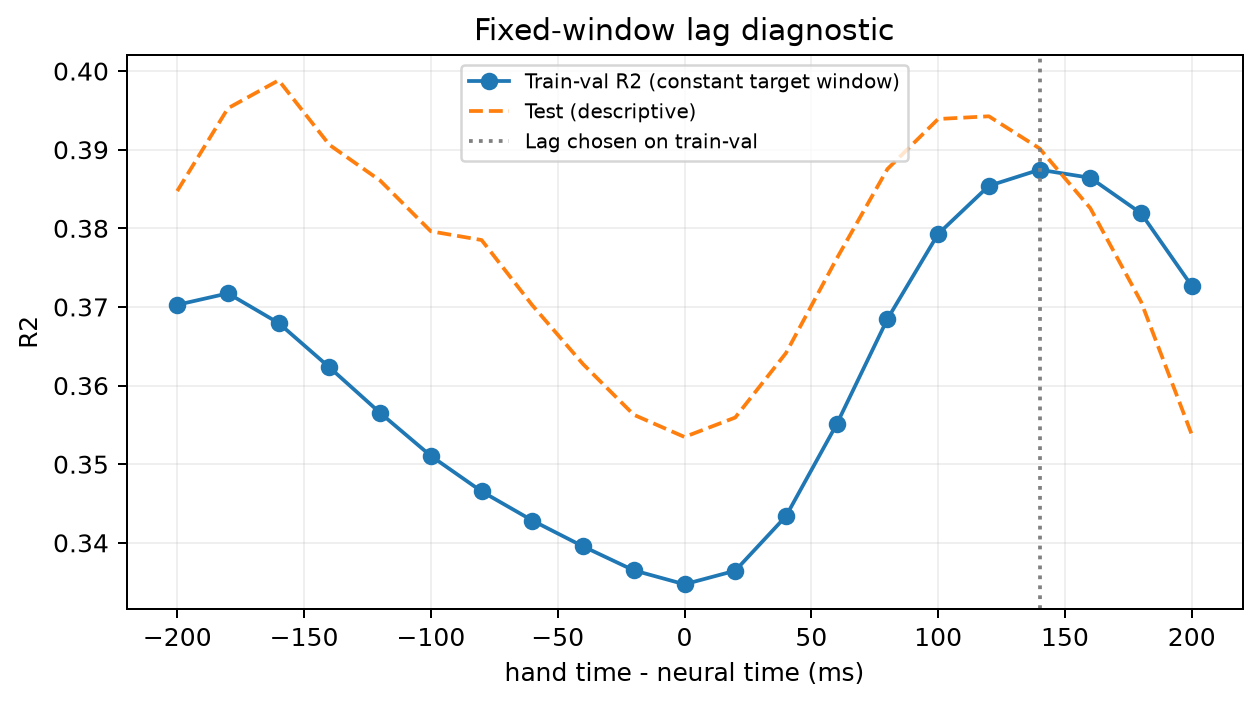
\includegraphics[width=0.93\textwidth]{fixed_window_lag.png}
\caption{固定手部评价时间窗后，神经时间偏移对 Ridge 预测 $R^2$ 的影响。纵轴为标准 $R^2$；实线是训练内部验证集，虚线测试曲线仅供诊断，不参与选择。}\label{fig:fixedlag}
\end{figure}
该现象\textbf{不能直接解释为 $140\,\mathrm{ms}$ 的真实神经生理传导时延}：运动准备、不同条件、平滑滤波、位置与速度混合，以及事件对齐方式均可能影响峰值位置。验证该机制需要更多因果/时序控制实验。特别是上述 Ridge 模型并不受 HiWA 正交约束，\textbf{这一结果不能直接算作 HiWA 的时间偏移改进}。

\subsection{关键诊断 C：原版均匀组质量与真实簇质量不符}
原版 HiWA 令四个簇各自的质量恒为 $1/4$；但真实 K-means 分组占比为
\begin{equation}
 \pi_X\approx(0.296,0.308,0.225,0.172),\qquad
 \pi_Y\approx(0.201,0.451,0.144,0.204).
\end{equation}
目标域第二簇约占全部时窗 $45.1\%$，与原版强加的 $25\%$ 差距明显。均匀簇质量对于这个数据不是经验频率模型。由于 HiWA 还独立从每簇抽取相同数量样本，组内、组间的概率解释与完整真实分布存在偏差。

把训练集已知时间对应仅用于\emph{事后诊断}，记录神经簇与行为簇的共现矩阵。即使允许四个簇做最佳一对一置换，能落在对应簇对里的同步窗口也只有约 \textbf{51.1\%}。这不是分类准确率，也不能用来取代 rMSE/$R^2$；它说明四个源簇与四个目标簇\textbf{未必存在清晰的一对一分组关系}。

\begin{figure}[H]\centering
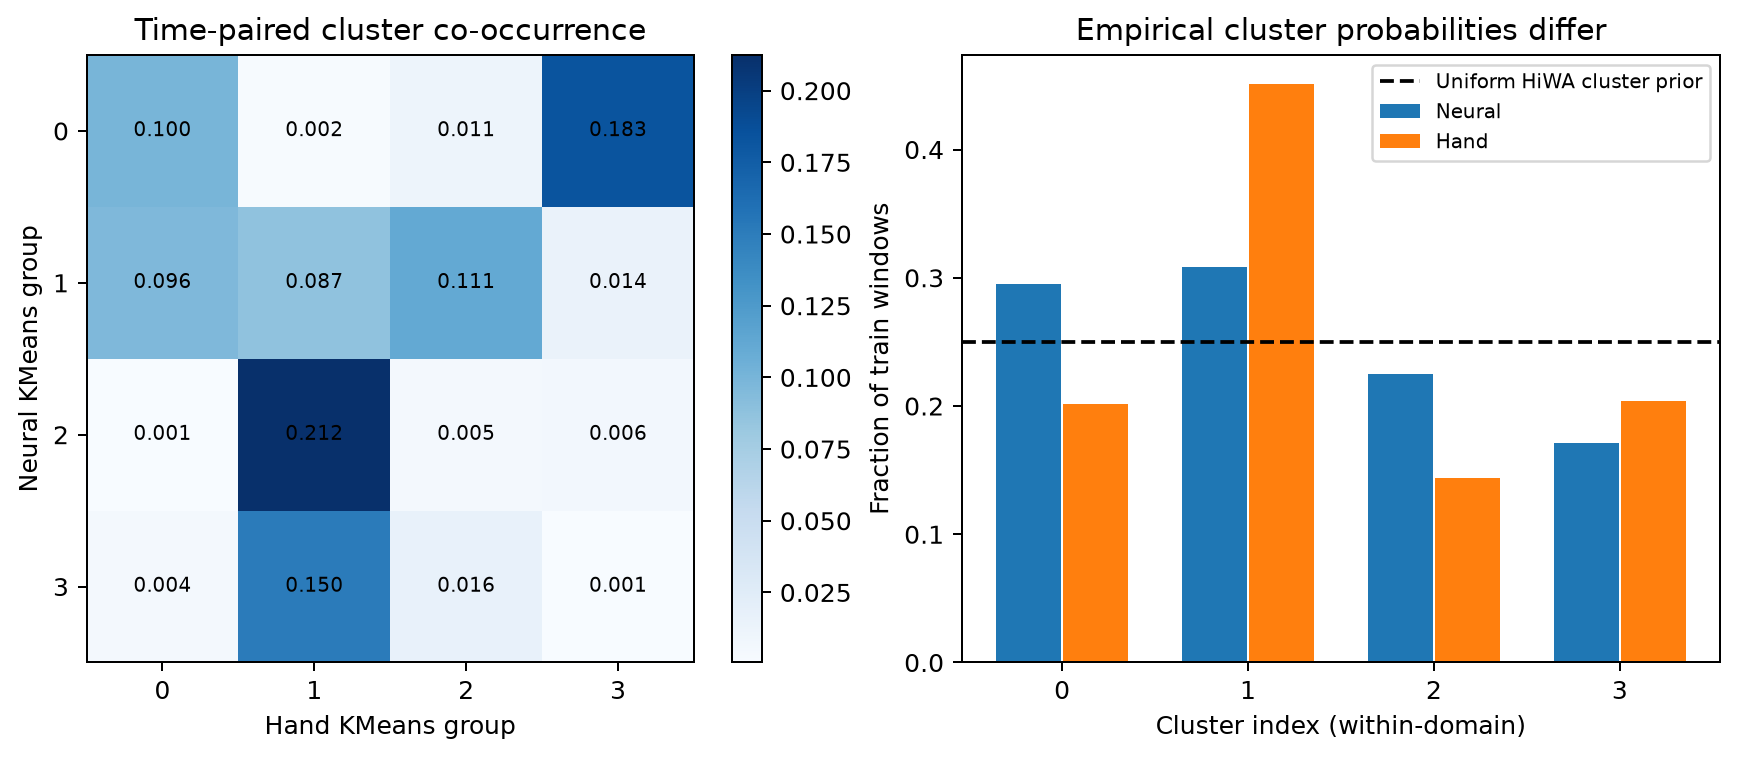
\includegraphics[width=0.97\textwidth]{cluster_masses_and_cooccurrence.png}
\caption{左：根据真实时间配对计算的簇共现概率（仅诊断）；右：两域经验簇质量与 HiWA 固定的均匀 0.25 质量比较。}\label{fig:group}
\end{figure}

\subsection{关键诊断 D：不同种子可能落入不同的等价/局部几何配置}
不同种子恢复的 $P$ 对四个目标簇的偏好排列不同。若事后与同步簇共现矩阵比较，种子 42--46 所选择的主簇置换分别覆盖约 $32.0\%$、$50.8\%$、$28.7\%$、$24.2\%$、$17.7\%$ 的同步窗口。它们不稳定；不能将低 OT 代价自动解释为恢复了稳定的语义对齐。

同时 seed 42 的 $\det(\widehat R)\approx-1$，其他四次约 $+1$。这是原版数学约束 $O(4)$ 允许的反射，而非浮点程序报错。若科研目标真正要求\emph{保持取向}的旋转，应将 $SO(4)$ 约束作为\textbf{后续独立消融实验}，不能在当前声称忠实复现原版的实验中悄悄修改。

\section{现阶段判断与下一个研究问题}
\subsection{已经确认的事实与尚未证明的推断}
\begin{itemize}
\item \textbf{事实：}原始 162 维神经放电的四维 PCA 表示与原生四维手部位置/速度已完成读取、独立硬聚类和原版 Hard HiWA 的五次运行；数值审计通过。
\item \textbf{事实：}在同一评价口径下，Hard HiWA 的留出测试 $R^2$ 全为负，而利用同步训练配对拟合的一般四维线性模型给出正的测试 $R^2$。
\item \textbf{事实：}组质量明显不均匀；簇对应关系不是稳定的一对一匹配；仅靠当前正交约束难以取得满意结果。
\item \textbf{推断：}正交等距模型和时间配准是目前更有证据支持的障碍；PCA 信息损失、聚类粒度、组质量设定也可能共同影响结果。
\item \textbf{尚未证明：}原始 HiWA 代码存在数值实现错误；$140$ ms 是真实生理延迟；软分组一定优于硬分组。上述三者都需要新的对照实验。
\end{itemize}

\subsection{下一阶段的优先验证顺序}
\begin{enumerate}[leftmargin=2.5em,itemsep=4pt]
\item \textbf{固定主评价指标：}继续记录代理 rMSE 和标准 $R^2$，解释代理 rMSE 的定义局限；诊断图、收敛检查不作为第三个性能指标。
\item \textbf{分清表征与映射限制：}在试次严格分离前提下，比较原始四维 PCA、替代的有监督神经维度选择和更高维神经子空间。若仅全线性有效、正交持续失效，应修改数学研究假设，而非单纯增加 Sinkhorn 迭代。
\item \textbf{验证时间因素：}把 $\ell$ 仅在训练验证中选择，再重新运行同条件的 HiWA 并评估测试，分清固定评价窗口、位置/速度分量和神经准备期带来的影响。
\item \textbf{检验组的统计含义：}独立比较 $K$ 与不均匀组权重的变体；分别记录跨种子 $P$、$R$ 稳定性。此实验属于\textbf{扩展方法}，不能混入原版 HiWA 的基线。
\end{enumerate}

\noindent\textbf{凝练后的研究问题：}对于 \emph{非等距、非同步且组质量不均衡}的神经--运动两个域，如何构造可解释、可识别并能够在留出试次上泛化的分层最优传输对齐模型？

\section*{复现文件与参考资料}
\addcontentsline{toc}{section}{复现文件与参考资料}
\noindent\textbf{项目目录：}\repo。\par
\begin{sloppypar}\noindent\textbf{代码入口：}\path{code/run_hard_clustering.py}（预处理及硬聚类），\path{code/hiwa_original.py}（原版求解器），\path{code/run_hard_hiwa.py}（对齐），\path{code/evaluate_hiwa_two_metrics.py}（两个主指标）。\par\noindent\textbf{新增诊断：}\path{code/diagnose_hiwa.py}、\path{code/diagnose_fixed_window_lag.py}、\path{code/diagnose_group_structure.py}。原始 NWB 需从 DANDI 下载，不上传 Git。\end{sloppypar}
\vspace{5pt}
\noindent [1] DANDI Archive. \emph{MC\_Maze\_Large} (DANDI:000138), v0.220113.0407.\\\url{https://dandiarchive.org/dandiset/000138/0.220113.0407}\par
\noindent [2] Neural Latents Benchmark, MC\_Maze datasets and task description.\\\url{https://neurallatents.github.io/datasets}\par
\noindent [3] Pei et al. \emph{Neural Latents Benchmark '21: Evaluating latent variable models of neural population activity}. NeurIPS Datasets and Benchmarks, 2021.\\\url{https://openreview.net/pdf?id=KVMS3fl4Rsv}\par
\noindent [4] 用户上传的原始复现包（2026-10-18）与其 PyHiWA 源码，及本项目 2026-11-17 冻结的 GitHub 数值记录。\par
\end{document}
